%%%%%%%%%%%%%%%%%%%%%%%%%%%%%%%%%%%%%%%%%
% Arsclassica Article
% LaTeX Template
% Version 1.0 (21/4/14)
%
% This template has been downloaded from:
% http://www.LaTeXTemplates.com
%
% Original author:
% Lorenzo Pantieri (http://www.lorenzopantieri.net) with extensive modifications by:
% Vel (vel@latextemplates.com)
%
% License:
% CC BY-NC-SA 3.0 (http://creativecommons.org/licenses/by-nc-sa/3.0/)
%
%%%%%%%%%%%%%%%%%%%%%%%%%%%%%%%%%%%%%%%%%

%----------------------------------------------------------------------------------------
%	PACKAGES AND OTHER DOCUMENT CONFIGURATIONS
%----------------------------------------------------------------------------------------

\documentclass[
10pt, % Main document font size
letterpaper, % Paper type, use 'letterpaper' for US Letter paper
oneside, % One page layout (no page indentation)
%twoside, % Two page layout (page indentation for binding and different headers)
headinclude,footinclude, % Extra spacing for the header and footer
BCOR5mm, % Binding correction
]{scrartcl}

%%%%%%%%%%%%%%%%%%%%%%%%%%%%%%%%%%%%%%%%%
% Arsclassica Article
% Structure Specification File
%
% This file has been downloaded from:
% http://www.LaTeXTemplates.com
%
% Original author:
% Lorenzo Pantieri (http://www.lorenzopantieri.net) with extensive modifications by:
% Vel (vel@latextemplates.com)
%
% License:
% CC BY-NC-SA 3.0 (http://creativecommons.org/licenses/by-nc-sa/3.0/)
%
%%%%%%%%%%%%%%%%%%%%%%%%%%%%%%%%%%%%%%%%%

%----------------------------------------------------------------------------------------
%	REQUIRED PACKAGES
%----------------------------------------------------------------------------------------

\usepackage[
nochapters, % Turn off chapters since this is an article        
beramono, % Use the Bera Mono font for monospaced text (\texttt)
eulermath,% Use the Euler font for mathematics
pdfspacing, % Makes use of pdftex’ letter spacing capabilities via the microtype package
dottedtoc % Dotted lines leading to the page numbers in the table of contents
]{classicthesis} % The layout is based on the Classic Thesis style

\usepackage{arsclassica} % Modifies the Classic Thesis package

\usepackage[T1]{fontenc} % Use 8-bit encoding that has 256 glyphs

\usepackage[utf8]{inputenc} % Required for including letters with accents

\usepackage{graphicx} % Required for including images
\graphicspath{{Figures/}} % Set the default folder for images

\usepackage{enumitem} % Required for manipulating the whitespace between and within lists

\usepackage{lipsum} % Used for inserting dummy 'Lorem ipsum' text into the template

\usepackage{subfig} % Required for creating figures with multiple parts (subfigures)

\usepackage{amsmath,amssymb,amsthm} % For including math equations, theorems, symbols, etc

\usepackage{varioref} % More descriptive referencing

%----------------------------------------------------------------------------------------
%	THEOREM STYLES
%---------------------------------------------------------------------------------------

\theoremstyle{definition} % Define theorem styles here based on the definition style (used for definitions and examples)
\newtheorem{definition}{Definition}

\theoremstyle{plain} % Define theorem styles here based on the plain style (used for theorems, lemmas, propositions)
\newtheorem{theorem}{Theorem}

\theoremstyle{remark} % Define theorem styles here based on the remark style (used for remarks and notes)

%----------------------------------------------------------------------------------------
%	HYPERLINKS
%---------------------------------------------------------------------------------------

\hypersetup{
%draft, % Uncomment to remove all links (useful for printing in black and white)
colorlinks=true, breaklinks=true, bookmarks=true,bookmarksnumbered,
urlcolor=webbrown, linkcolor=RoyalBlue, citecolor=webgreen, % Link colors
pdftitle={}, % PDF title
pdfauthor={\textcopyright}, % PDF Author
pdfsubject={}, % PDF Subject
pdfkeywords={}, % PDF Keywords
pdfcreator={pdfLaTeX}, % PDF Creator
pdfproducer={LaTeX with hyperref and ClassicThesis} % PDF producer
} % Include the structure.tex file which specified the document structure and layout


\usepackage{listings}
\usepackage{xcolor}
\usepackage{color}

\definecolor{mygray}{rgb}{0.4,0.4,0.4}
\definecolor{mygreen}{rgb}{0,0.8,0.6}
\definecolor{myorange}{rgb}{1.0,0.4,0}

\lstset{language=C++,
       basicstyle=\ttfamily\scriptsize,
       keywordstyle=\color{blue}\ttfamily,
       stringstyle=\color{red}\ttfamily,
       commentstyle=\color{green}\ttfamily,
       numbers=left,
       numbersep=5pt,
       numberstyle=\tiny\color{mygray},
       breaklines=true
      }

\newcommand{\fix}[1]{\texttt{\small #1}}

\hyphenation{Fortran hy-phen-ation} % Specify custom hyphenation points in words with dashes where you would like hyphenation to occur, or alternatively, don't put any dashes in a word to stop hyphenation altogether

%----------------------------------------------------------------------------------------
%	TITLE AND AUTHOR(S)
%----------------------------------------------------------------------------------------

\title{\normalfont\spacedallcaps{Evaluation Segmentation on GPUs}} % The article title

\author{\spacedlowsmallcaps{Abdul Dakkak}} % The article author(s) - author affiliations need to be specified in the AUTHOR AFFILIATIONS block

\date{} % An optional date to appear under the author(s)

%----------------------------------------------------------------------------------------

\begin{document}

%----------------------------------------------------------------------------------------
%	HEADERS
%----------------------------------------------------------------------------------------

\renewcommand{\sectionmark}[1]{\markright{\spacedlowsmallcaps{#1}}} % The header for all pages (oneside) or for even pages (twoside)
%\renewcommand{\subsectionmark}[1]{\markright{\thesubsection~#1}} % Uncomment when using the twoside option - this modifies the header on odd pages
\lehead{\mbox{\llap{\small\thepage\kern1em\color{halfgray} \vline}\color{halfgray}\hspace{0.5em}\rightmark\hfil}} % The header style

\pagestyle{scrheadings} % Enable the headers specified in this block

%----------------------------------------------------------------------------------------
%	TABLE OF CONTENTS & LISTS OF FIGURES AND TABLES
%----------------------------------------------------------------------------------------

\maketitle % Print the title/author/date block

\setcounter{tocdepth}{2} % Set the depth of the table of contents to show sections and subsections only


%----------------------------------------------------------------------------------------
%	ABSTRACT
%----------------------------------------------------------------------------------------

\section*{Abstract} % This section will not appear in the table of contents due to the star (\section*)

Image segmentation is an important and well studied problem in computer vision.
The task is to label pixels, grouping them into the same category.
In medical imaging, for example, one needs to classify a liver from the rest of 
  the image, or discern the shape of cells to detect any diseases.
Sadly, segmentation is slow --- taking on the order of minutes.
Speeding up segmentation would not only improve existing applications, but 
  also open the possibility of new ones.

In this project we evaluate image segmentation on the GPU.
We look at Cellular Automaton (CA) based 
  approaches for binary segmentation (classifying pixels as either background
  or foreground).
We try different optimizations on both CPUs and GPU and perform a comparison.

%----------------------------------------------------------------------------------------
%	AUTHOR AFFILIATIONS
%----------------------------------------------------------------------------------------

\let\thefootnote\relax\footnotetext{* \textit{dakkak@illinois.edu}}

%----------------------------------------------------------------------------------------

%\newpage % Start the article content on the second page, remove this if you have a longer abstract that goes onto the second page

 

%----------------------------------------------------------------------------------------
% GrowCut
%----------------------------------------------------------------------------------------

\section{Cellular Automaton (GrowCut) Based Segmentation}

GrowCut~\cite{vezhnevets2005growcut} is an algorithm that uses ideas from cellular automaton to perform image
  segmentation.
GrowCut flood
  neighbors based on an initial seed until it reaches a barrier.
One can think of each pixel as a bacteria with an energy function, if a bacteria has
  higher energy than one of its neighbors, then it will devour them --- otherwise it
  is the victim.
The algorithm is iterated until either a fixed point is reached or the maximum number
  of iterations are reached.
A pseudocode of the algorithm is shown in listing~\ref{lst:growcut}.
For our experiments, we set \fix{MAX\_ITERATIONS} to $2048$ and use a
  penalty function $g(x,y)  = 1 - \|x - y\|_2$.


\lstinputlisting[language=C++, caption=Pseudo Code for GrowCut Segmentation, label={lst:growcut}]{code/growcut.cu}

\subsection{Markov Random Field (GraphCut) Based Segmentation}

MRF have been used in GPU computing with good success.
The problem is that they do not map nicely to the hardware --- use
  irregular data structures, require atomic updates, etc...
Furthermore, the method is patented which limits its usefulness in 
  real world applications.
While we initially had an MRF implementation, we abandoned it
  in favor of a much more interesting algorithm that maps nicely to
  GPUs.

\subsection{Optimizations}

In this section we evaluate different optimizations on both CPUs and GPUs.


\paragraph{Task Based Parallelization}
We first parallelized the code to run on different CPU cores.
This was done using a task based approach (using Thread Building Blocks~\cite{reinders2007intel}) 
  which simplifies some of the programming.

\paragraph{Base CUDA Implementation}
Once the threaded multi-core version was working, we ported the code to use CUDA. 
Each thread in CUDA processes a pixel, access its elements, and updates its state.
A global synchronization is required after each iteration of the algorithm since boundary edges are not known after a thread group completes.

\paragraph{CUDA Implementation Using Shared Memory}
Shared memory are memory residing on each core of the GPU. Placing reused memory there, instead of always accessing it of chip, is a common optimization.
In place of explicitly computing the $2$-norm, we use the \fix{hypotf} function in this step as an added optimization.
We also give compile hints so constant memory are to be placed in a constant memory space (which is a separate part of the hardware dedicated to read-only memory).

\paragraph{Approximating the $2$-norm}
The $2$-norm computation is the only complicated arithmetic operation in our code, we therefore substituting it by using the fact that $\|x-y\|_2$ can be approximated
with $\alpha Max(x,y) + \beta Min(x,y)$, the choice of $\alpha$ and $\beta$ depend on the error you can tolerate. We chose $\alpha = 1$ and $\beta = 1/2$ which gives
a maximum error of $11.8\%$ and a mean error of $8.86$ on average.

\paragraph{Approximating the Algorithm}
A synchronization is required between iterations different iterations of the algorithm.
Since CUDA has no global synchronization capabilities, we essentially do a local 
  synchronization (within the block).
To not propagate error too much, we perform $32$ iterations before doing a global synchronization.

Since the value of boundary pixels is not known within a local synchronization, we 
  make the assumption that boundary pixels ``look'' like their neighbors or their 
  previous state.
If both the past history and the neighbors match, then we keep the value unchanged.
Otherwise, we have a $50\%$ probability to be correct and take the value of the
  neighborhood pixel.
Figure~\ref{fig:approx} shows the effects of this approximation.


\begin{figure}[tb]
\centering
\subfloat[True Solution]{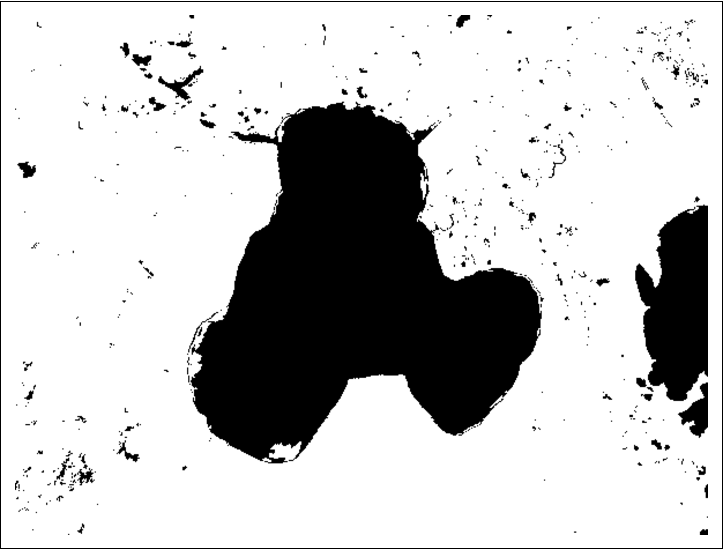
\includegraphics[width=.3\columnwidth]{figs/true.pdf}} \quad%
\subfloat[Approximate Solution]{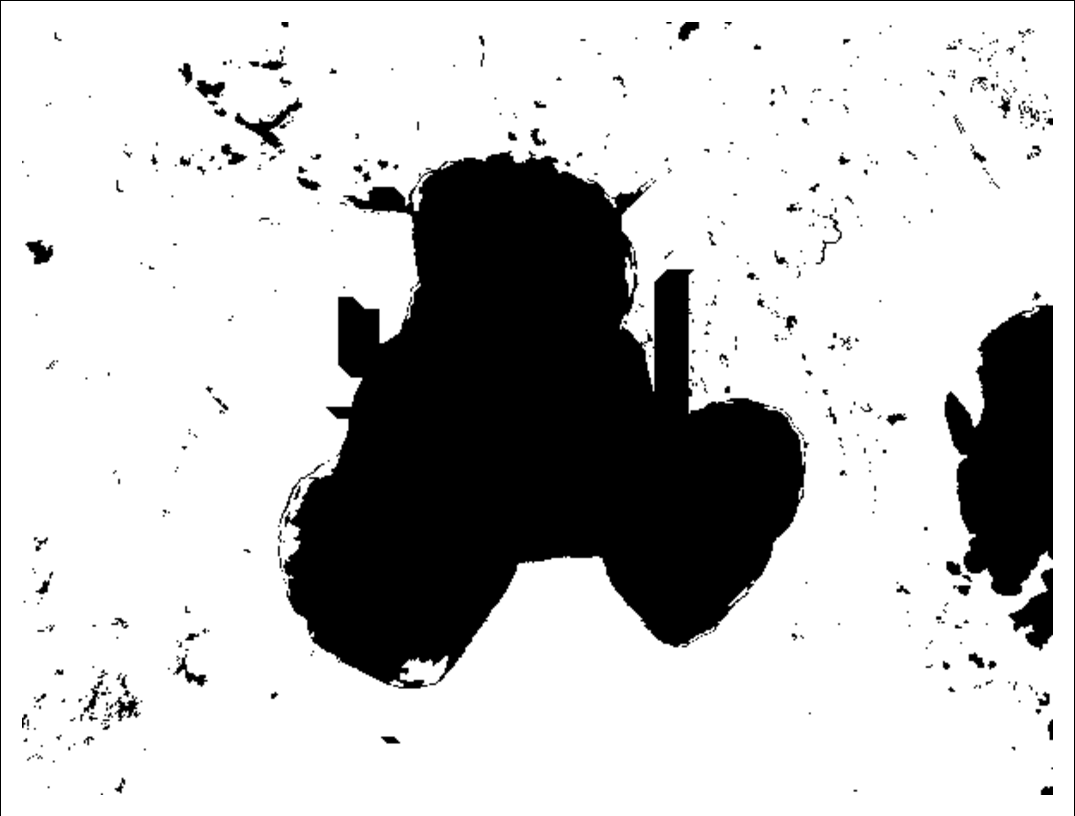
\includegraphics[width=.3\columnwidth]{figs/approx.pdf}} \quad%
\subfloat[Error]{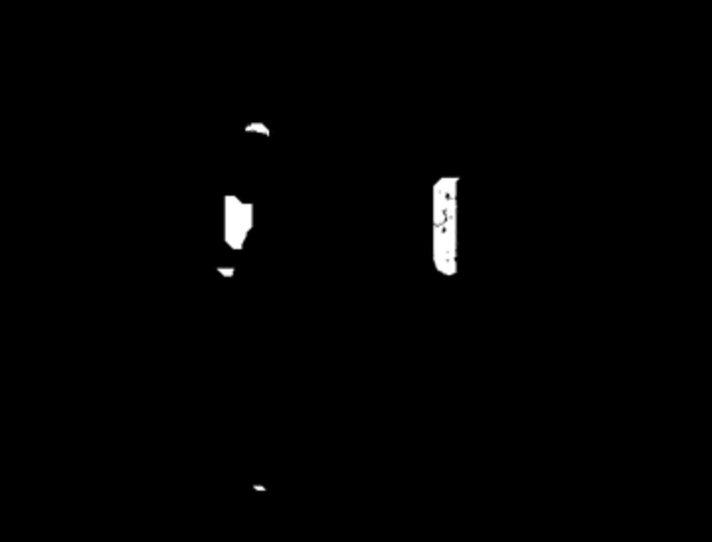
\includegraphics[width=.3\columnwidth]{figs/error.pdf}}
\caption{This shows the effects of approximating the algorithm by not having a global synchronization after each step. We rescale our differences so that even small errors are visable.}
\label{fig:approx}
\end{figure}

%----------------------------------------------------------------------------------------
%	METHODS
%----------------------------------------------------------------------------------------

\section{Evaluation}


\begin{figure}[tb]
\centering 
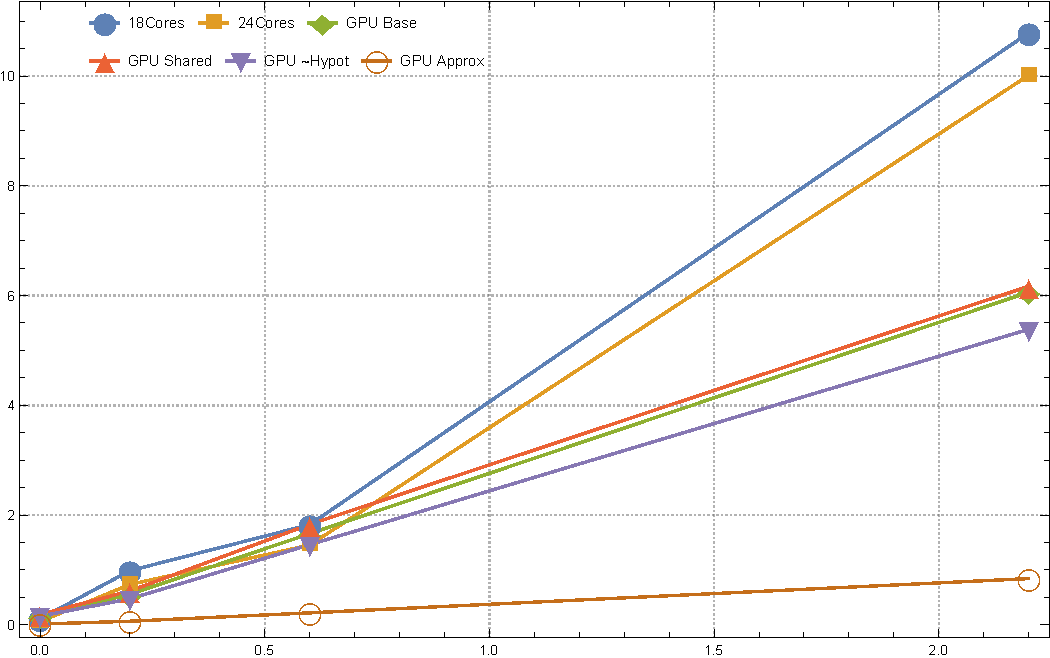
\includegraphics[width=\columnwidth]{figs/perf.pdf} 
\caption{This shows the timing of GrowCut on a $24$ and $32$ core system.
As expected, no difference is noticed between the two configurations due to hitting I/O
bandwidth limits. The $x$ axis is the number of megapixels in the image and the $y$ axis is the execution time in seconds. It also shows the effects of different GPU optimizations.}
\label{fig:growcut} 
\end{figure}

In Figure~\ref{fig:growcut} we see that having $24$ core (Intel Xeon X5660) vs $32$ core (Intel Xeon X5675) does not make a difference for streaming, since
  one hits the memory and I/O bandwidth limits (and essentially encounters Amdahl's law).
More advanced configurations, such as RAID, would allow us to scale better as the number of cores become large.

Figure~\ref{fig:growcut} shows the effects of different GPU optimizations on a C2070 GPU.
The GPU base version performs the computation using an $8 \times 8$ work group.
The GPU shared version places the $label$, $strength$, and $image$ data into 
  shared memory before performing the computation.
Since error can be tolerated, the GPU $\sim$Hypot version approximates
  the $2$-norm using the  ``$\alpha$-max plus $\beta$-min algorithm'' with
  $\alpha = 1$ and $\beta = 1/2$.
The final version, GPU Approx, introduces more error by performing multiple iterations without doing a global synchronization.
This shows that beyond program tuning for hardware, one can exploit the error tolerance for this class of algorithms to achieve great speedup.


%----------------------------------------------------------------------------------------
% FUTURE
%----------------------------------------------------------------------------------------

\section{Future Work}

One key observation in segmentation is that the labeling is decided in the
  first few iterations of the algorithm.
A simple optimization to reduce our error while approximating the algorithm is to
  start the algorithm with a global synchronization after each iterations (computing
  the true solution).
At some time $t$ we can more safely perform the approximation by having global synchronization after $n$ iterations of the algorithm.
At a later time $t+s$, we can perform the synchronization after $2n$ iterations.



%----------------------------------------------------------------------------------------
%	BIBLIOGRAPHY
%----------------------------------------------------------------------------------------

\renewcommand{\refname}{\spacedlowsmallcaps{References}} % For modifying the bibliography heading

\bibliographystyle{unsrt}

\bibliography{paper}



%----------------------------------------------------------------------------------------
% APPENDIX
%----------------------------------------------------------------------------------------
\newpage


\section{Appendix}

\lstinputlisting[language=C++, caption=Final optimized and approximated code, label={lst:growcut}]{code/growcut_cuda_opt_4.cu}

%----------------------------------------------------------------------------------------

\end{document}